\documentclass[twocolumn]{article}
\usepackage[utf8]{inputenc}
\usepackage[T1]{fontenc}
\usepackage[ngerman]{babel}
\usepackage{fancyhdr}
\usepackage{geometry}
\usepackage[table]{xcolor}
\usepackage{amsmath}
\usepackage{amssymb}
\usepackage{tabularx}
\usepackage{listings}
\usepackage{lstautogobble}
\usepackage{graphicx}
\usepackage{wrapfig}

\geometry{
    a4paper,
    top=30mm,
    bottom=30mm,
    left=20mm,
    right=20mm,
}

\newcommand*{\qed}{\hfill\ensuremath{\square}}

\pagestyle{fancy}
\fancyhf{}
\lhead{AaS-Benchmark}
\rhead{Alexander Korn}
\rfoot{\thepage}

\title{\Large \textbf{Übersicht über die Funktionalität von AaS-Benchmark mit Beispielen}}
\author{Alexander Korn}
\date{}

\begin{document}

\maketitle

\tableofcontents

\section{Einleitung}

\textit{AaS-Benchmark} ist ein Tool, das es ermöglicht, die Ausführungszeiten von Algorithmen aus der Vorlesung \textit{Algorithmen auf Sequenzen} zu messen. Dabei können verschiedenste Parameter gewählt werden, um so beispielsweise Zusammenhänge von Musterlängen und Ausführungszeiten zu erkennen. Die Algorithmen aus der Vorlesung sowie dieses Tool wurden dazu in der Programmiersprache \textit{Rust} implementiert.

In dieser Übersicht sollen dem Leser die verschiedenen Funktionen von AaS-Benchmark nähergebracht und mit einigen Beispielen demonstriert werden.

Das Tool lässt sich auf GitHub 

\section{Algorithmen}

Für Aas-Benchmark wurden elf Algorithmen aus der Vorlesung implementiert. Diese lassen sich wie folgt in drei Kategorien aufteilen:

\subsection{Algorithmen für einzelne Muster}

Diese Gruppe von Algorithmen findet alle Vorkommen eines einzelnen Musters in einem Text. Implementiert sind in dieser Gruppe die folgenden Algorithmen:

\begin{itemize}
    \item Naiver Algorithmus
    \item Knuth-Morris-Pratt
    \item Shift-And
    \item Backward Nondeterministic DAWG Matching (BNDM)
    \item Backward Oracle Matching (BOM)
\end{itemize}

\subsection{Algorithmen für mehrere Muster}

Diese Gruppe enthält Algorithmen, die alle Vorkommen von Mustern aus einer gegebenen Menge in einem Text finden. Sie unterscheiden sich also insofern von den Algorithmen der letzten Gruppe, als dass sie nicht mit nur nach einem einzelnen Muster suchen, sondern nach mehreren Mustern gleichzeitig.

Hier sind ein naiver Algorithmus sowie der \textit{Aho-Corasick} Algorithmus implementiert.

\subsection{Fehlertolerante Algorithmen}

Fehlertolerante Algorithmen sind solche, die ein Muster in einem Text finden können, wobei das Muster allerdings nicht exakt den Vorkommen im Text entsprechen muss. Es lässt sich hierbei ein maximal gewünschter Fehler angeben, das heißt ein Wert, welcher aussagt, wie viele Abweichungen bei Vorkommen des Musters im Text vorhanden sein dürfen.

Eine Abweichung beschreibt die Einfügung, Löschung oder Ersetzung eines Zeichens in einer im Text gefundenen Zeichenkette, um diese an das zu findende Muster anzunähern.

Als fehlertolerante Algorithmen sind die fehlertolerante Variante des Shift-And Algorithmus sowie \textit{Ukkonens} DP Algorithmus implementiert.

\subsection{Volltextindizes}

Für diese Kategorie sind zwei Arten von Algorithmen implementiert. Die einen dienen der Konstruktion eines Volltextindexes, während die anderen Muster in einem Text mittels des vorher erzeugten Volltextindexes suchen.

Ein Volltextindex ist eine Datenstruktur, welche aus einem Text erzeugt werden kann und es ermöglicht, verschiedene Operationen effizienter durchführen zu können, als hätte man lediglich den Text.

Als Volltextindex-Datenstruktur ist das \textit{Suffix Array} implementiert, das mittels eines naiven Algorithmus oder des sehr schnellen, in Linearzeit ausführbaren, \textit{SAIS}-Algorithmus erzeugt werden kann. Zur Mustersuche mittels eines Suffix Arrays sind Algorithmus zur exakten Mustersuche, sowie der \textit{Backward-Search}-Algorithmus implementiert. Letzterer benötigt zusätzlich zum Suffix Array auch noch die \textit{Burrows-Wheeler-Transformation} und die \textit{Occ}- und \textit{Less}-Arrays benötigt. Auch diese drei Datenstrukturen lassen sich mit Aas-Benchmark zur Ausführung des oben genannten Algorithmus erzeugen.

\section{Das Ausgabeformat}

Wurde Aas-Benchmark korrekt ausgeführt, erhält man eine Ausgabe, die der Form der in Listing \ref{lst:output_format_example} gezeigten Daten entspricht. Diese Ausgabe hat das CSV Format, es handelt sich also um eine Tabelle, bei der die Spalten je Zeile durch Kommata getrennt sind. Die erste Zeile enthält dabei den Tabellenkopf.

Jede Zeile steht für eine einzelne Ausführung des Algorithmus, der in der ersten Spalte der Zeile gegeben ist. Die Spalten enthalten die folgenden Informationen:

\begin{itemize}
    \item \texttt{algorithm}: Der ausgeführte Algorithmus
    \item \texttt{text\_length}: Die Länge des Textes bei dieser Ausführung
    \item \texttt{pattern\_length}: Die Länge des Musters bei dieser Ausführung
    \item \texttt{execution}: Die wievielte Ausführung dies ist
    \item \texttt{matches}: Wie viele Vorkommen des Musters bei dieser Ausführung im Text gefunden wurden
    \item \texttt{prep\_time\_ms}: Die benötigte Vorbereitungszeit in Millisekunden\footnote{Bei Algorithmen, die keine Vorbereitungszeit benötigen, immer 0}
    \item \texttt{time\_ms}: Die benötigte Zeit, um den Algorithmus mit den gegebenen Parametern auszuführen
\end{itemize}

\lstinputlisting[caption=Beispiel des Ausgabeformates, captionpos=b, frame=single, breaklines=true, label=lst:output_format_example]{assets/output_format_example.csv}

\section{Beispiele}

Beginnen wir mit einem einfachen Beispiel. Wir möchten testen, wie sich die Laufzeit des naiven Algorithmus für die Mustersuche bei steigender Musterlänge verhält.

Der Befehl für die Ausführung von AaS-Benchmark könnte dafür zum Beispiel wie folgt aussehen:

\begin{lstlisting}[breaklines=true,autogobble=true]
    ./aas-benchmark naive -t 100000000 -p 1..10
\end{lstlisting}

\begin{figure}
    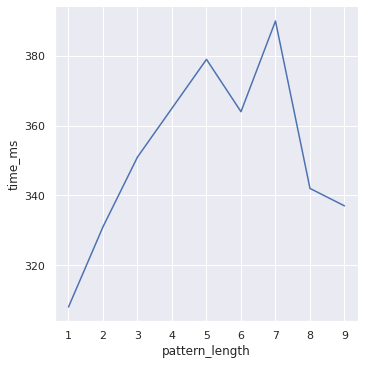
\includegraphics[width=\linewidth]{assets/graph_1.png}
    \caption{Laufzeit des naiven Algorithmus}
    \label{fig:runtime_naive}
\end{figure}

Lässt man sich die Ausgabe dieses Befehls plotten, so erhält man das Diagramm in Abbildung \ref{fig:runtime_naive}. So kann man mit Aas-Benchmark das Verhalten der implementierten Algorithmen einfach betrachten und die verschiedenen Algorithmen miteinander vergleichen.

Als nächsten schauen wir uns ein einfaches Beispiel an, bei dem die Laufzeit zweier Algorithmen bei steigender Musterlänge geprüft wurde. Dazu wurde der folgende Befehl verwendet:

\begin{lstlisting}[breaklines=true,autogobble=true]
    ./aas-benchmark kmp,horspool -t 100000000 -p 1..10
\end{lstlisting}

\begin{figure}
    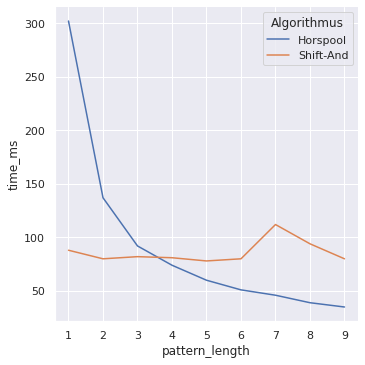
\includegraphics[width=\linewidth]{assets/graph_2.png}
    \caption{Laufzeit des Horspool Algorithmus verglichen mit der des Shift-And Algorithmus}
    \label{fig:runtime_horspool_shift_and}
\end{figure}

Lässt man sich die Ausgabe erneut plotten (Abbildung \ref{fig:runtime_horspool_shift_and}), kann man nun erkennen, dass der \textit{Horspool} Algorithmus mit steigender Musterlänge immer schneller ausgeführt werden kann, während die Laufzeit des \textit{Shift-And} Algorithmus relativ konstant bleibt.

Dies gilt hier, da auf einem Text mit einer Länge von 100.000.000 Zeichen gesucht wird, bei dem selbst eine 

Nun möchten wir testen, wie sich die Laufzeit eines Algorithmus verhält, wenn wir ihn mehrmals hintereinander mit den gleichen Paramtern, also auf dem gleichen Text mit dem gleichen zu findenden Muster, ausführen.

\end{document}
